\documentclass[../../Aurora C# unofficial manual.tex]{subfiles}

\begin{document}
	\section{Surface-to-Orbit weapons}
	Original post can be found
	\href{http://aurora2.pentarch.org/index.php?topic=8495.msg110500#msg110500}{here}.
	\\\\
	
	A ground unit class has an option to mount a surface-to-orbit component. If this option is selected, the class must also select a weapon type. The weapon can be of any type researched by the owning race, including turrets and spinal weapons. Additional systems will be automatically added based on the weapon chosen, creating an integrated component (similar in concept to CIWS). These systems include:
	
	\textbf{Beam Fire Control:} For normal weapons, this will be created using options for 4x Racial Fire Control Range and 1x Racial Tracking Speed. If the Point Defence Weapon checkbox is clicked, the fire control will be created using options for 1x Racial Fire Control Range and 4x Racial Tracking Speed. In all cases, the beam fire control will have a 25\% range bonus vs a ship-mounted equivalent. The cost and size of the fire control will be 50\% of the ship version due to its dedication to a single weapon.
	
	\textbf{Active Sensor:} This sensor will be resolution 1 and have range at least equal to the maximum range of the weapon. The minimum size will be 5 tons. The sensor is fully functional and will detect targets in general, not just for the weapon. Size and cost are normal.
	
	\textbf{Reactor:} This component will be designed to generate sufficient power for the weapons capacitor. Size and cost are normal.
	
	\textbf{ECCM:} This is optional and can be added by checking Include ECCM checkbox. Size is 50 tons and cost is half normal to reflect the dedication to a single weapon.
	
	Those ground elements containing units with STO capability can set a number of different targeting options. For the moment, targeting and firing is handled automatically although I may add a manual targeting option as well. For those targeting options directed at ships, the player may also select the number of weapons per target, with zero being all weapons. When a number other than zero is chosen, the targets are cycled until all weapons are fired. Targets must be detected, hostile and in range to be eligible.
	
	The target settings are as follows:
	\begin{itemize}
		\item Do Not Fire
		\item Target Random Ship:  Eligible Ships are given a random order and the targeting cycles though them (or targets the first if number of weapons is zero). The targets will be cycled through multiple times if required for all weapons to fire.
		\item Target Largest Ship:  Eligible Ships are arranged in descending order of size
		\item Target Smallest Ship:  Eligible Ships are arranged in ascending order of size
		\item Target Fastest Ship:  Eligible Ships are arranged in descending order of speed
		\item Target Slowest Ship:  Eligible Ships are arranged in ascending order of speed
		\item Target Easiest Ship:  Eligible Ships are arranged in descending order of chance to hit
		\item Target Shipyards:  The largest eligible shipyard contact is targeted
		\item Target Populations:  The largest eligible population contact is targeted. Populations on the same system body as the STO element cannot be targeted.
		\item Target Ground Forces:  The largest eligible ground forces contact is targeted. Ground forces on the same system body as the STO element cannot be targeted.
		\item Target STO Ground Forces:  The largest eligible STO ground forces contact is targeted. STO ground forces on the same system body as the STO element cannot be targeted.
		\item Final Defensive Fire:  When a salvo is about to hit a target within range of the STO weapon, the element will be eligible for point defence fire in the same way as a ship. This allows the STO element to protect itself and other ground forces, any populations on the surface, orbital shipyards and any nearby ships.
		\item Final Defensive Fire (Surface Only):  Same as Final Defensive Fire except that only salvos attacking surface targets will be intercepted
		\item Area Point Defence:  The STO units will shoot at any hostile missiles currently in range.
	\end{itemize}

	When an STO element targets missiles, it will only fire until the missiles are destroyed. For the purposes of tracking weapon fire and recharging, each STO unit within the element is tracked separately.
	\begin{figure}[H]
		\centering
		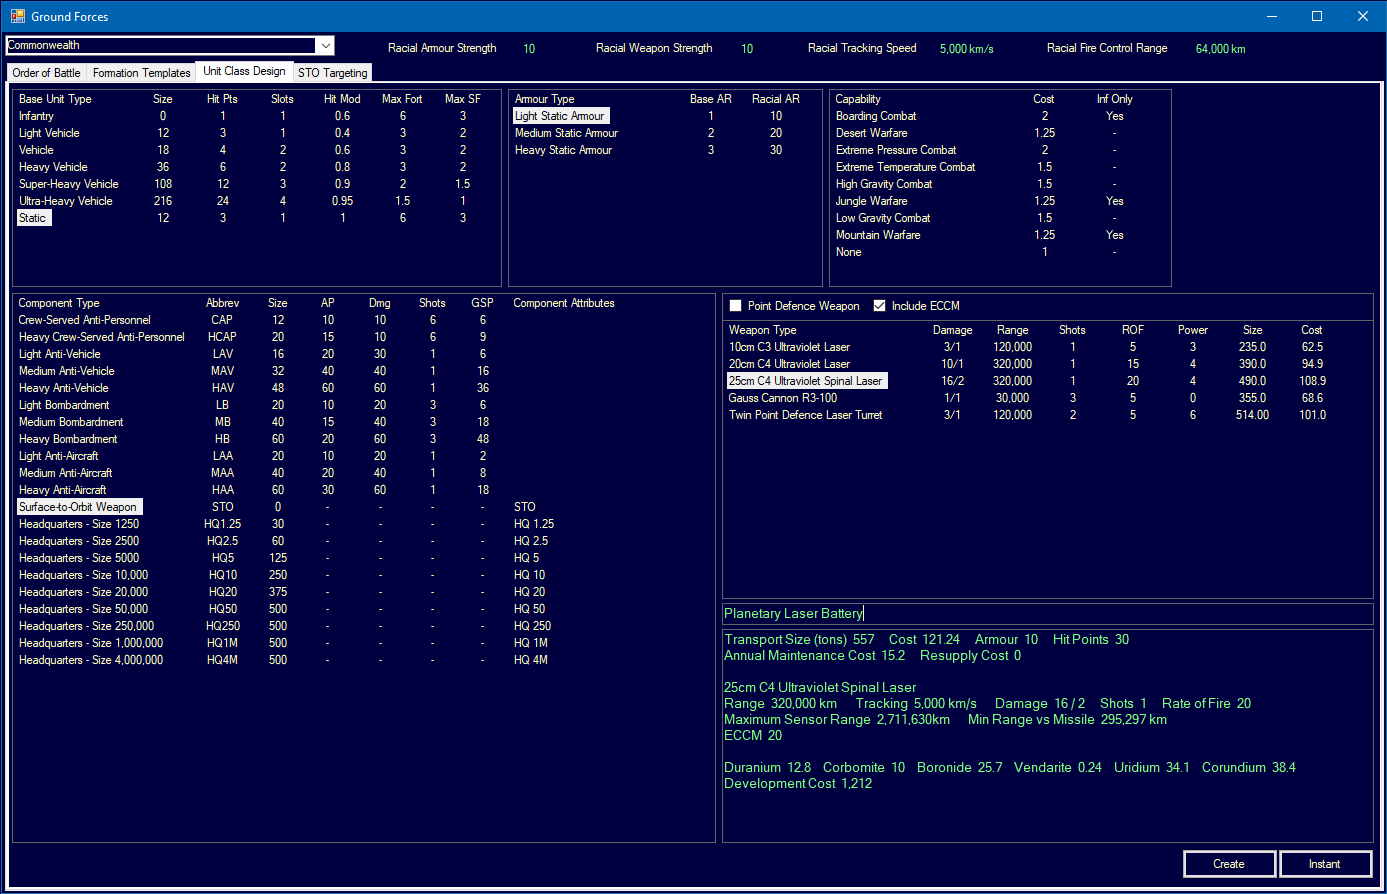
\includegraphics[width=0.95\linewidth]{images/STOWeapons}
		\caption[STO Weapons]{Surface-to-Orbit Weapons Example 1}
		\label{fig:stoweapons}
	\end{figure}
	\begin{figure}[H]
		\centering
		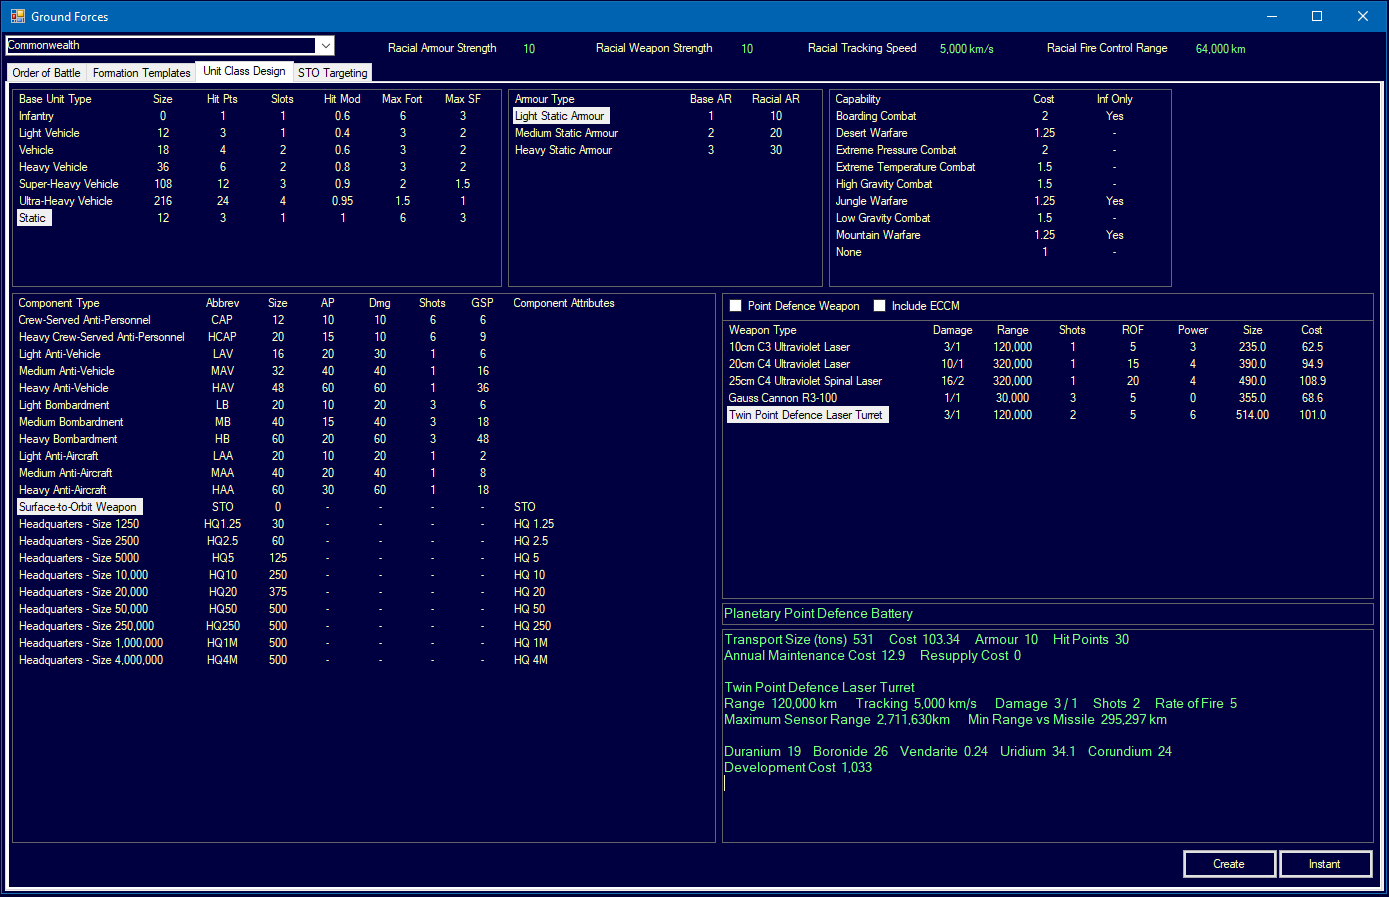
\includegraphics[width=0.95\linewidth]{images/STOWeapons2}
		\caption[STO Weapons]{Surface-to-Orbit Weapons Example 2}
		\label{fig:stoweapons2}
	\end{figure}
\end{document}